\documentclass[runningheads]{llncs}

\usepackage{caption} % change the font size of figure captions.
\captionsetup[figure]{font=small}
\usepackage{graphicx}
\usepackage{array}
\usepackage{booktabs}
\usepackage{float}
\usepackage{hyperref}
\usepackage{amsmath}
\usepackage{float}
\usepackage{subcaption}
\usepackage{color}

\renewcommand\UrlFont{\color{blue}\rmfamily}
% ---- Statistics ----- %
% abstract: 132
% Introduction: 554
% Related Work: 589

\begin{document}
    \title{Automatic Evaluation of Generative Dialogue Systems: An Empirical Study}
    \titlerunning{Automatic Evaluation of Generative Dialogue Systems}
    \author{Cong Feng \and Wenge Rong \and Jianxin Yang \and Haodong Yang \and \\Yuanxin Ouyang \and Zhang Xiong}
    \authorrunning{Feng et al.}
    \institute{
    School of Computer Science and Engineering, Beihang University, Beijing, China
    \email{\{congfeng, w.rong, yjx17, yhd125, oyyx, xiongz\}@buaa.edu.cn}
    }

    \maketitle

    % --------------------------- %
    % --------- Abstract -------- %
    % --------------------------- %
\begin{abstract}
Evaluating generative dialogue systems with automatic metrics is a challenging task. It has been shown that the word-overlap metrics such as BLEU and the word-embedding metrics do not correlate well with human judgements. Furthermore, regardless of the correlation with human judgments, the scores of these metrics do not correlate well with others, which means fine-tuning a dialogue system on one set of metrics may yield inconsistency when testing with another set of metrics. This infeasibility again adds to the ineffectiveness of evaluation dialogue systems. To the end of utilizing metrics at its best, in this research, we offer several pragmatic suggestions on the use of automatic metrics to avoid the issue of metric inconsistency by empirically evaluating a set of automatic evaluation metrics.
\keywords{Automatic Evaluation Metrics, Dialogue Response Generation, Chatbot}
\end{abstract}

    % ----------------------------------- %
    % ---------- Introduction ----------- %
    % ----------------------------------- %
\section{Introduction}
%The chat-oriented dialogue systems have seen a boom in the recent literature of dialogue systems. These systems are trained to make an appropriate response given a conversational context and can be applied to various chatbot applications, language education tools, and intelligent personal assistants. This setting is different from that of the traditional task-oriented dialogue systems, which are programmed to assist their users to complete a certain task, such as restaurant reservation and airline information acquisition. As a result, the chat-oriented dialogue systems cannot be evaluated in the same supervised setting as their task-oriented counterpart, which turns out to bring a new challenge.

%As an advanced approach to the chat-oriented system, the generative models based on neural networks feature end-to-end training with minimal hard-coded features and the ability to output fluent human-like sentences. Given a large corpus of context-response pairs, these neural models can learn language patterns and extract common-sense knowledge from the corpus in an unsupervised manner, making it a highly plausible solution to the response generation problem.

%Vinyals et al. \cite{GoogleChatbot} applied the

Recently the chat-oriented dialogue systems have seen a boom in the community. These systems are trained to make an appropriate response given a conversational context and can be applied to various applications. One of the fundamental technique in such dialogue systems is generative model, which can learn language patterns and extract knowledge from the corpus in an unsupervised manner. The research community has made steady progress with the generative models and one of the most widely used techniques is Seq2Seq model \cite{Seq2Seq}. Though generative models have shown promising result, there exist one essential challenge. They incline to give meaningless responses to the questions, e.g., \textit{I don't know}, thereby making their evaluation remain an open problem \cite{HowNot}.

Currently most generative dialogue systems are evaluated by borrowing automatic metrics from other tasks, e.g., machine translation, such as the BLEU \cite{BLEU}, METEOR \cite{METEOR} and etc. However, the correlations between these borrowed metrics and human judgments were unclear and researchers generally fell back to human evaluation for better accuracy and reliability \cite{VHRED,Shang}. It is found that those metrics only correlated weakly with human judgments on the non-technical Twitter corpus and not at all on the technical Ubuntu Dialogue Corpus \cite{HowNot}, which calls for new automatic metrics that are more relevant to human judgments.

In this paper, we followed the previous work and further investigated the behaviors of automatic metrics without human judgments. We analyzed both system-level and example-level scores to find out possible correlations among different metrics. In particular, we drew samples from the example-level scores of different metrics and analyze the pairwise correlation of these samples. It is found that some pairs of samples have a high correlation, while other pairs show a much lower one.

Following these observations, we further clustered the metrics based on the pairwise correlations of their corresponding samples. The results show that similar metrics tend to cluster together, indicating a high pairwise correlation within the same group. According to the experiment results, it is argued that the scores given by dissimilar metrics have the risk of high inconsistency, which is yet another pitfall of using automatic metrics. Therefore, it is strongly recommended to choose consistent metrics for the ease of comparison across different settings.

    % ----------------------------------- %
    % ----------- Related Work ---------- %
    % ----------------------------------- %
\section{Related Work}
%Previous works on automatic metrics have mostly focused on the correlation between the metrics and human judgments. After all, the advantages of automatic metrics would be largely compromised if they cannot reflect human judgments. For example, in machine translation, where automatic metrics have been established to reduce human labor, almost every newly proposed metrics report an improved human correlation, as in \cite{NIST}, \cite{METEOR}, and \cite{chrf}.

In dialogue response generation, to address the issue of low metric-human correlation, various semantic-based methods have been proposed. For example, the ADEM metric proposed models the human judgments with a feed-forward neural network \cite{ADEM}. The RUBER metric takes an asymmetric approach w.r.t the response-context pair and response-reference pair, where the former is modeled by a neural network and the latter is measured by an embedding-based metric. They combined two scores with various heuristics and achieved improvements on a Chinese corpus \cite{RUBER}. In brief, correlation with human judgments has been the supervised signal guiding the evolution of automatic metrics.

Other popular metrics include perplexity, which is generally used to evaluate statistical language models. Vinyals et al. revealed that their Seq2Seq dialogue model achieved a much lower perplexity than the n-gram baseline, but they also admitted the drawbacks of using such a metric \cite{GoogleChatbot}. Serban et al. also used perplexity to evaluate their models \cite{HRED}, along with other metrics. However they were also not clear about how well these metrics accounted for the grammatical correctness and semantic coherence of the responses.

Generally, automatic metrics have been constantly doubted of their capability to reflect human judgments. In one of the earliest attempts to the response generation problem, Ritter et al. made an initial examination on the suitability of BLEU to this field leveraging the human data they collected \cite{Ritter11}. They found that the BLEU scores were very low even on the system level and the correlation was modest. Similarly, Shang et al. also argued that BLEU did not apply as the reasonable responses evaluation \cite{Shang}.

%Their study took into account of various settings, such as both retrieval and generative models and both technical and non-technical datasets. 

An extensive study of metric-human correlation was conducted by Liu et al. \cite{HowNot}. It was revealed that although these metrics could distinguish state-of-art models from baseline models, none of them correlated highly with human scores. Their work has left us two questions: 1) How can we improve the metric-human correlation? 2) Why do the existing metrics correlate badly with human judgments? Previous works that proposed enhanced metrics endeavored to answer the first question, while we try to shed some light on the second one. In particular, we are curious about what can we learn when scores from different metrics are put together and compared across various settings.

%To understand why some metrics correlate poorly with human judgments, we show that there are general inconsistencies among these metrics. Intuitively, if a set of metrics have low pairwise correlations, it is less likely that all of them would correlate highly with human judgments, which indicates that some of them must correlate poorly with human judgments. Along this line of thought, we arrive at an intermediate explanation to the poor performance of automatic metrics, backed by an empirical study. With this in mind, we can partially understand why these metrics fail and make improvements from the lesson we learned.

    % ----------------------------------- %
    % --------- Experiment Setup -------- %
    % ----------------------------------- %
\section{Experiment Configuration}
Our experiment essentially involves training multiple generative models on multiple datasets, and then measure their performances with various automatic metrics. As stated, our study does not involve human evaluation. We also do not consider retrieval models as we mainly focuse on generative models. Due to the time and resource constrains, we limit our scope to three commonly used models and three datasets.

%To ease our demonstration, we define some symbols. A \emph{model} denoted by $m$ is an architecture of generative models, not an \emph{instance} of model trained on a specific dataset. A \emph{dataset} denoted by $d$ is a collection of context-response pairs from a specific domain, such as a social media or a technical support forum. A \emph{metric} denoted by $s$ is a function mapping a segment of tokens to a real value. The segment can be a sentence or a collection of sentences. $(m, d)$ denotes a model instance of architecture $m$ trained on dataset $d$.

    % ------------------------- %
    % --------- Metrics ------- %
    % ------------------------- %
\subsection{Metrics}
Here are a list of popular metrics used in dialogue response evaluation included in this research.%    We extend the set of metrics studied by \cite{HowNot} with some new ones from the recent literature, namely ADEM \cite{ADEM} and Distinct-N \cite{MMI}. We make a quick review on these metrics.

1) BLEU \cite{BLEU} is a classical metric for machine translation that reports a high correlation with human scores on the system level. It owes the quality of a hypothesis to its similarity to multiple references. It computes the geometric mean of consecutive orders of n-gram precision, multiplied by a brevity penalty.

\iffalse
    \begin{align}
        p_n &= \frac{ |C_n \cap R_n| }{ |R_n| } \\
        \textit{BP} &=
        \begin{cases}
            \ 1 \ & \text{if} \  c > r \\
            \ e^{1 - r/c} \ & \text{otherwise} \\
        \end{cases} \\
        \textit{BLEU} &=
        \textit{BP} \cdot \exp \left( \sum_{n=1}^N w_n \log p_n \right)
    \end{align}
    $p_n$ is the n-gram precision for order $n$. $C_n$ is a multiset of n-gram from a hypothesis while $R_n$ is the union of multisets of n-gram from each reference. $\textit{BP}$ is the brevity penalty. $c$ and $r$ are the length of the hypothesis and the effective length\footnote{The effective length of a collection of references is the length closest to that of the hypothesis.} of the references, respectively. $N$ is the total number of orders and a common choice is 4. $w_n$ is a weighting factor that usually takes the uniform weight $1 / N$.
\fi

2) METEOR \cite{METEOR} is a metric proposed to address several issues with BLEU. It applies multiple stages of unigram matching to the hypothesis and reference, each using a different criterion, such as exact matching, WordNet synonyms, and paraphrases. An alignment is then created from these unigram matches. The score is based on the F1 of the alignment and a penalty to shorter matches.

3) ROUGE \cite{ROUGE} is a family of metrics for automatic summarization. It is based on the F1 score and can integrate different counting units, e.g., n-gram statistics and the longest common subsequence. 

\iffalse
The common form of ROUGE is:
    \begin{align}
        \textit{ROUGE} = \frac{
        R \cdot P
        }{(1 - \alpha) P + \alpha R}
    \end{align}
    where $R$ and $P$ and the recall and precision, respectively. $\alpha$ controls the relative importance of $R$ and $P$. It should be a large value if only recall is considered.
\fi

4) Embedding Average is a metric based on word embedding, a distributed approach to the meaning of words \cite{word2vec}. The embedding of a sentence is defined as the average of the embeddings of its composing words. The similarity of two sentences is then simply defined as the cosine of the corresponding vectors.

5) Vector Extrema \cite{Vector_Extrema} composes the sentence embedding by taking the most extreme value (either maximum or minimum) along each dimension from its constitutive words. The intuition is that in the embedding space, common words like function words are pulled towards the origin as they appear in the context of many different words, while informative words are pushed away from the origin in either positive or negative direction, since they tend to appear in more specific context. %By taking the most extreme values, this method essentially captures more informative words and ignore common words.

6) Greedy Matching \cite{GreedyAndOptimal} is an embedding-based method without calculating a sentence vector. Instead, two sentences under comparison are treated as a weighted bipartite graph, taking their words as nodes and the embedding cosine of two words $\cos(w, w')$ as the edge weight. The metric is based on a greedy method to solve the optimal matching problem on the weighted graph:
    \begin{align}
        G(r, \hat{r}) = \frac{
        \sum_{w \in r} \max_{\hat{w} \in \hat{r}} \cos(e_w, e_{\hat{w}})
        }{ |r| } \\
        \textit{Greedy-Matching} = \frac{
        G(r, \hat{r}) + G(\hat{r}, r)
        }{2}
    \end{align}
    where $r$ and $\hat{r}$ are the reference and response, respectively.

7) ADEM \cite{ADEM} is an approach based on a concise nueral network. The model first embeds a context $c$, response $\hat{r}$, and reference $r$ into a low-rank vector space and then predicts the human score with a linear combination of the input features:
    \begin{align}
        s(c, r, \hat{r}) = \frac{(c^T M \hat{r} + r^T N \hat{r} - \alpha)}{\beta}
    \end{align}
    $M, N$ are learnable parameters of the network and $\alpha, \beta$ are constants to normalize the output to a five-point score. The model is trained on a human-annotated conversation corpus to minimize the squared error with L2 regularization:
    \begin{align}
        L = \sum_{i=1}^{K} (s_i - h_i)^2 + \gamma \left\| \theta \right\| _2
    \end{align}
    where $K$ is the number of samples in a batch. $s_i$ and $h_i$ are the model prediction and the human score, respectively. $\theta$ is the parameters of the network and $\gamma$ is the regularization factor.

8) Distinct-N \cite{MMI} measures the rate of unique n-grams of a sentence. For a sentence, it is the number of unique n-grams divided by the total number of n-grams. It is a token-level measurement of the diversity of a response.

    % ------------------------- %
    % --------- Models -------- %
    % ------------------------- %
\subsection{Models}
In our research, three representative models from \cite{VHRED} are selected, namely LSTM, HRED, and VHRED. LSTM is a simple model based on the Long Short-Term Memory \cite{LSTM}. HRED extends the standard Seq2Seq framework by using a hierarchical encoder. VHRED is an extension to HRED that injects randomness into the decoder to achieve higher diversity. As such, they form a hierarchy of architectural sophistication and are ideal baselines of generative models.

1) The LSTM model is a simple generative model with a single RNN acting as both an encoder and a decoder. Note that the generative LSTM is not an autoregressive model as the output of the previous time step does not become the input of the current time step.

%For an input sequence $X = x_1, x_2, \dots, x_n$ and an output sequence $Y = y_1, y_2, \dots y_m$, the model predicts $y_t$ conditioned on $x_t$ at time step $t$.

2) The HRED model \cite{hred-qs,HRED} features a hierarchical encoding mechanism that takes into account the structure of dialogues. It first encodes each sentence with an \emph{utterance encoder} into a fixed-length utterance vector $e_u$. Then, the utterance vectors are processed iteratively by the \emph{context encoder} to produce a fixed-length context vector $e_d$. Finally, the \emph{utterance decoder} takes the context vector and generates the next utterance of the dialogue. %With the hierarchical generation process, it can better incorporate long-term dialogue history and generate more topic-relevant resposnes \cite{A_Short_Review}.

3) The VHRED model \cite{VHRED} extends the HRED model with a variational inference mechanism. Essentially, VHRED injects into the utterance decoder random variables that are sampled from a high-dimension normal distribution, the parameters of which are conditioned on the context vector $e_d$. %With the randomness at the decoder, VHRED is able to model the uncertainty and ambiguity in the dialogues, generating more diverse responses \cite{A_Short_Review}.

%\subsubsection{Training Procedure.}
    The configurations for different model components are shown in Table \ref{tab:model_config}. We used Adam \cite{AdamOpt} as our optimizer and applied gradient clipping with a threshold of 1. The learning rate was set to 0.0002 on the Ubuntu corpus and 0.0002 on the others. All the models were trained on a Nvidia GTX for at least one week. We used random sampling when testing.
    \begin{table}
    \centering
    \caption{Model Configuration}
    \label{tab:model_config}
    \begin{subtable}{0.5\textwidth}
        \centering
        \caption{Utterance Encoder}
        \begin{tabular}{|l|r|r|}
            \hline
            & {Embedding} & {\#Hidden Units} \\
            \hline
            LSDSCC & 400 & 1000 \\
            \hline
            OpenSubtitles & 400 & 1000 \\
            \hline
            Ubuntu & 300 & 500 \\
            \hline
        \end{tabular}
    \end{subtable}%
    \begin{subtable}{0.45\textwidth}
        \centering
        \caption{Context Encoder}
        \begin{tabular}{|l|r|r|}
            \hline
            & RNN Direction & \#Hidden Units \\
            \hline
            LSDSCC & bidirectional & 1000 \\
            \hline
            OpenSubtitles & bidirectional & 1000 \\
            \hline
            Ubuntu & unidirectional & 1000 \\
            \hline
        \end{tabular}
    \end{subtable}
    \begin{subtable}{\textwidth}
        \centering
        \caption{Utterance Decoder}
        \begin{tabular}{|l|*{7}{r|}}
            \hline
            & \multicolumn{3}{c|}{RNN Type}
            & \multicolumn{3}{c|}{\#Hidden Units} \\
            \hline
            & HRED & LSTM & VHRED & HRED & LSTM & VHRED \\
            \hline
            LSDSCC & LSTM & GRU & GRU & 1000 & 2000 & 1000 \\
            \hline
            OpenSubtitles & LSTM & GRU & GRU & 1000 & 2000 & 1000 \\
            \hline
            Ubuntu & LSTM & LSTM & LSTM & 500 & 2000 & 500 \\
            \hline
        \end{tabular}
    \end{subtable}
\end{table}

    % --------------------------- %
    % --------- Datasets -------- %
    % --------------------------- %
\subsection{Datasets}
In this research, we select three commonly used datasets, the statistics of which are listed in table \ref{tab:dataset_stats}. These datasets represent three common domains in the literature, namely technical support, movie subtitles and online forums.
    \begin{table}[H]
    \centering
    \caption{Statistics of the Datasets}
    \label{tab:dataset_stats}
    \begin{tabular}{|*{8}{l|}}
        \hline
        & \multicolumn{4}{c|}{Training Set} & \multicolumn{2}{c|}{Testing Set} \\
        \hline
        & Vocabulary & \#Samples & \#Tokens & Turns & \#Samples & \#Tokens \\
        \hline
        Ubuntu & 20000 & 448833 & 45697699 & multiple & 18920 & 2045082   \\
        \hline
        OpenSubtitles & 23876 & 11771393 & 379346841 & multiple & 14714 & 474074 \\
        \hline
        LSDSCC & 35008 & 738095 & 32355628 & single & 299 & 10914 \\
        \hline
    \end{tabular}
\end{table}

1) The Ubuntu Dialogue Corpus \cite{ubuntu_corpus} is a large-scale multi-turn dyadic technical corpus collected from the Ubuntu channel of an IRC network\footnote{\url{https://irclogs.ubuntu.com/}}. It contains a lot of technical symbols, such as filesystem paths, commands, and URLs. %Its large-scale nature helps construct data-driven applications for technical support.

2) The OpenSubtitles dataset \cite{opensub} is an enormous corpus of movie subtitles. It is collected by the OPUS project \cite{OPUS} from the opensubtitles website\footnote{\url{http://www.opensubtitles.org}}. Typically, two consecutive utterances are treated as a context-response pair, as in \cite{GoogleChatbot,MMI}. %, and \cite{persona}.

%It is noisy as the examples are inherently not of dialogue structure. In other words, there are no explicit turn-taking information or dialogue boundaries in it. 

3) LSDSCC \cite{LSDSCC} is a domain-specific conversation corpus collected from the movie subreddit of the Reddit forum\footnote{\url{https://www.reddit.com/r/datasets}}. It is believed that a more specific domain can help avoid generating universal responses \cite{LSDSCC}. %The authors applied dedicated cleansing procedures to retain as much information as possible. They also used human annotations to ensure the quality of the corpus.

    % ------------------------------------- %
    % --------- Experimental Study -------- %
    % ------------------------------------- %
\section{Experimental Study}
\subsection{System-Level Scores}
We first measured the system-level scores for all settings, shown in Table \ref{tab:system_scores}. The system-level score reflects the average performance of a model trained on a dataset. For metrics that do not have an explicit system-level definition, we took the arithmetic average of their example-level scores.
\begin{table}%
    \centering%
    \caption{System-Level Scores for All Settings}%
    \small
    \label{tab:system_scores}%
    \setlength{\tabcolsep}{0.11cm}%
    \begin{tabular}{|l|r|r|r|r|r|r|r|r|r|}%
        \hline
        & \multicolumn{3}{c|}{LSDSCC} & \multicolumn{3}{c|}{OpenSubtitles} & \multicolumn{3}{c|}{Ubuntu}\\%
        \hline
        & HRED & LSTM & VHRE & HRED & LSTM & VHRE & HRED & LSTM & VHRE\\%
        \hline%
        ADEM & \textbf{2.6178} & 2.6127 & 2.6163 & \textbf{2.6228} & 2.6224 & 2.6219 & 2.6353 & \textbf{2.6381} & 2.635\\\hline
        BL{-}1 & \textbf{0.08} & 0.0726 & 0.0722 & 0.0672 & 0.0638 & \textbf{0.0753} & 0.1314 & 0.1303 & \textbf{0.1365}\\\hline
        BL{-}2 & \textbf{0.0264} & 0.0181 & 0.0185 & 0.0171 & 0.0153 & \textbf{0.0264} & 0.0362 & 0.0345 & \textbf{0.0375}\\\hline
        BL{-}3 & \textbf{0.0105} & 0.0052 & 0.0066 & 0.0062 & 0.0055 & \textbf{0.0146} & \textbf{0.009} & 0.007 & 0.0089\\\hline
        BL{-}4 & \textbf{0.0053} & 0.0 & 0.0028 & 0.0024 & 0.0022 & \textbf{0.01} & \textbf{0.0029} & 0.0018 & 0.0025\\\hline
        Dist{-}1 & \textbf{0.9577} & 0.9441 & 0.9558 & \textbf{0.973} & 0.9714 & 0.9714 & 0.9074 & \textbf{0.9257} & 0.9113\\\hline
        Dist{-}2 & \textbf{0.8541} & 0.8511 & 0.8497 & \textbf{0.8669} & 0.8594 & 0.8665 & \textbf{0.9013} & 0.8603 & 0.8968\\\hline
        Greedy & \textbf{0.3303} & 0.3292 & 0.3267 & 0.3102 & 0.2998 & \textbf{0.3145} & \textbf{0.2775} & 0.2364 & 0.273\\\hline
        Average & \textbf{0.5532} & 0.5467 & 0.5483 & 0.5453 & 0.5295 & \textbf{0.5485} & \textbf{0.574} & 0.5205 & 0.5655\\\hline
        Extrem & \textbf{0.2841} & 0.2835 & 0.2814 & 0.3009 & 0.2929 & \textbf{0.3061} & \textbf{0.29} & 0.2663 & 0.2875\\\hline
        MET & \textbf{0.0296} & 0.0258 & 0.0281 & 0.0248 & 0.0233 & \textbf{0.0271} & 0.1657 & 0.1635 & \textbf{0.166}\\\hline
        RO{-}1 & \textbf{0.108} & 0.083 & 0.0978 & 0.0784 & 0.075 & \textbf{0.0872} & 0.1644 & \textbf{0.1836} & 0.1683\\\hline
        RO{-}2 & \textbf{0.0226} & 0.0049 & 0.0081 & 0.0053 & 0.0043 & \textbf{0.0107} & 0.0128 & \textbf{0.0143} & 0.0128\\\hline
        RO{-}3 & \textbf{0.0057} & 0.0002 & 0.0035 & 0.0011 & 0.0009 & \textbf{0.0053} & \textbf{0.0007} & 0.0003 & 0.0005\\\hline
        RO{-}4 & 0.0011 & 0.0 & \textbf{0.003} & 0.0002 & 0.0002 & \textbf{0.0038} & \textbf{0.0002} & 0.0 & 0.0001\\\hline
        RO{-}L & \textbf{0.0956} & 0.0681 & 0.0846 & 0.0742 & 0.0707 & \textbf{0.0826} & 0.1493 & \textbf{0.1722} & 0.1535\\\hline
        RO{-}W & \textbf{0.0792} & 0.0537 & 0.07 & 0.066 & 0.0629 & \textbf{0.0734} & 0.1205 & \textbf{0.1391} & 0.1236\\\hline
        PPL & \textbf{32.5599} & 32.9229 & 37.7149 & 41.6392 & 34.2724 & \textbf{33.6867} & \textbf{39.178} & 46.4061 & 40.2641\\\hline
        \#words & 13.1605 & 14.0067 & 12.3612 & 8.807 & 8.6394 & 8.7798 & 23.0646 & 16.4905 & 21.2449\\
        \hline
        %
        %
    \end{tabular}
    %
\end{table}

The system-level scores of different metrics look quite consistent in terms of the best performing model on a certain dataset. On LSDSCC, for example, the HRED model beats all the other models on all but one metrics, while on OpenSubtitles, the VHRED model wins the best of most of the metrics. The system-level score seems to be able to distinguish state-of-the-art models from baselines, since most of the metrics agree on which model is the best.

    However, the consistency among the metrics does not necessarily lead to a high correlation with human judgment, as observed in \cite{HowNot}. Moreover, since the system-level score is calculated by accumulating over the example-level scores, it is possible that the inconsistency on the example-level is hidden away. To reveal the possible inconsistency, we performed analyses on the example-level scores.

    \subsection{Example-Level Scores}
    On the example level, a matrix $M \in R^{N \times M}$ is calculated for each model instance, where $N$ is the number of examples and $M$ is the number of metrics. Each row $r_i$ of the matrix is the scores of all metrics for an example $e_i$, while each column $c_j$ is the values of a metric $s_j$ computed for all examples. All the metrics share the same set of examples within a matrix. Thus, the correlation of any two columns $c_i, c_j$ can be understood as to how much the corresponding metrics $s_i, s_j$ agree on their shared examples. We compute the pairwise correlations of the metrics and highlight the degree of correlation with heatmaps, as shown in Fig. \ref{fig:corr_heatmap}. We used Pearson's r and all the results are statistically significant.

    \begin{figure}[htbp]
    \centering
    \begin{subfigure}{0.35\linewidth}
        \centering
        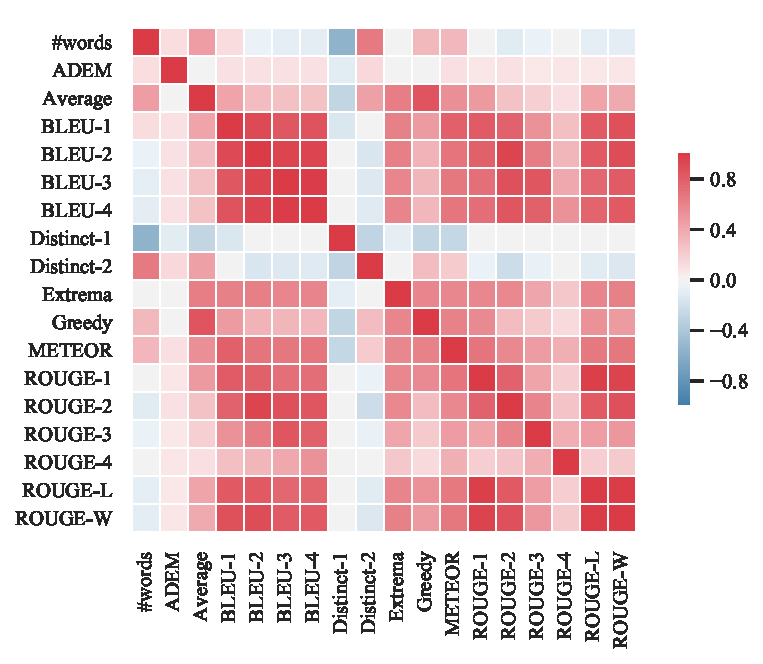
\includegraphics[width=\linewidth]{figure/plot/heatmap/v4/pearson/hred/lsdscc/plot.pdf}
        \caption{(HRED, LSDSCC)}
    \end{subfigure}%
    \begin{subfigure}{0.35\linewidth}
        \centering
        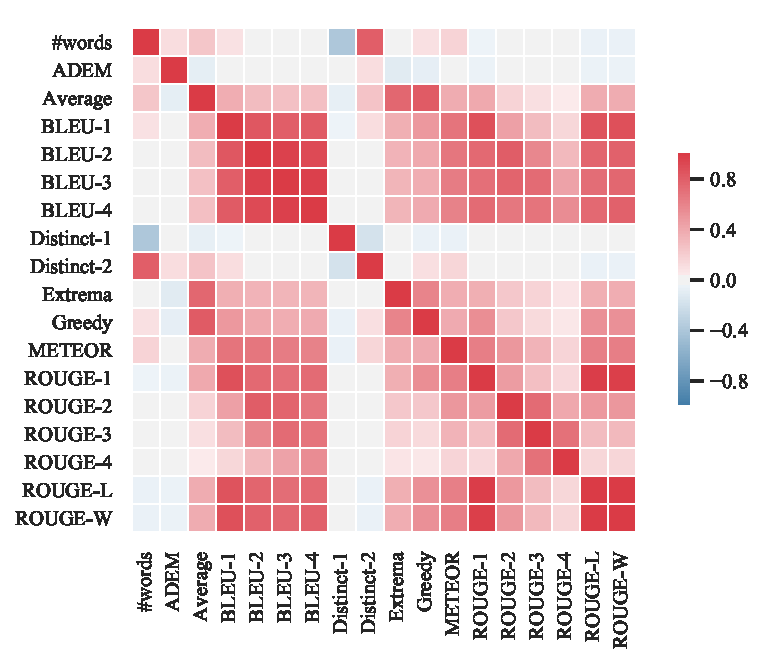
\includegraphics[width=\linewidth]{figure/plot/heatmap/v4/pearson/hred/opensub/plot.pdf}
        \caption{(HRED, OpenSubtitles)}
    \end{subfigure}%
    \begin{subfigure}{0.35\linewidth}
        \centering
        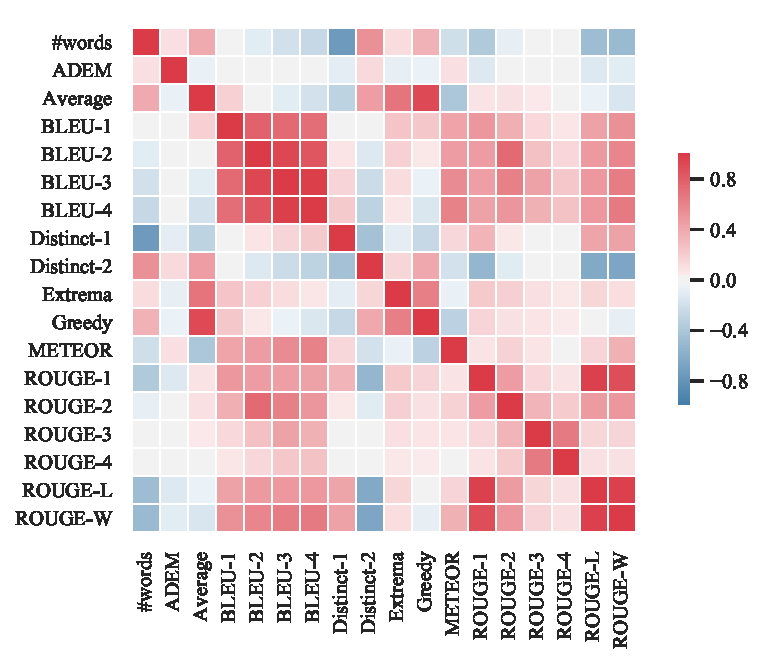
\includegraphics[width=\linewidth]{figure/plot/heatmap/v4/pearson/hred/ubuntu/plot.pdf}
        \caption{(HRED, Ubuntu)}
    \end{subfigure}
    \begin{subfigure}{0.35\linewidth}
        \centering
        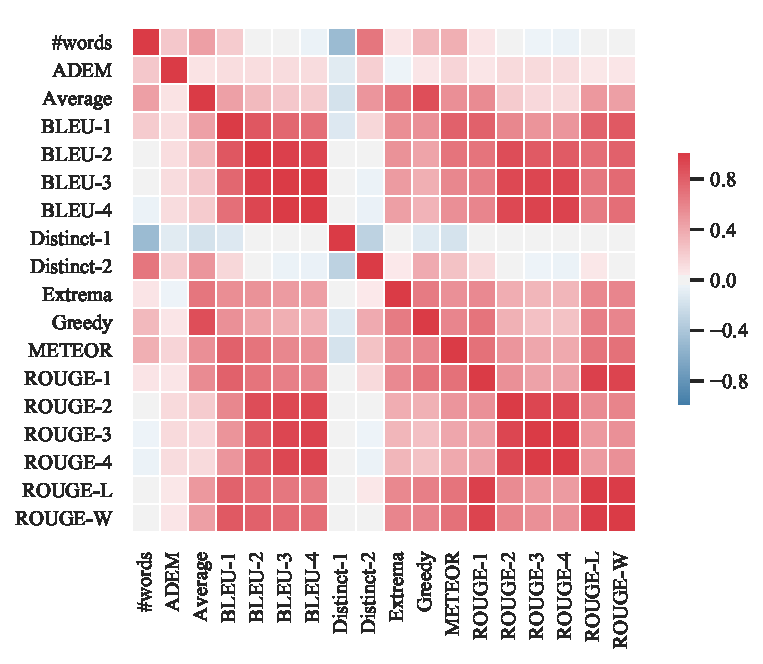
\includegraphics[width=\linewidth]{figure/plot/heatmap/v4/pearson/vhred/lsdscc/plot.pdf}
        \caption{(VHRED, LSDSCC)}
    \end{subfigure}%
    \begin{subfigure}{0.35\linewidth}
        \centering
        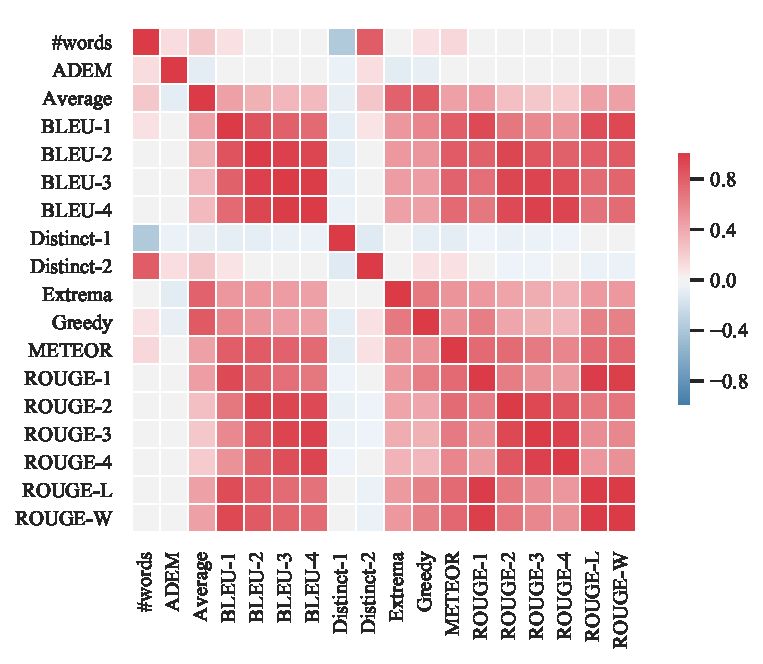
\includegraphics[width=\linewidth]{figure/plot/heatmap/v4/pearson/vhred/opensub/plot.pdf}
        \caption{(VHRED, OpenSubtitles)}
    \end{subfigure}%
    \begin{subfigure}{0.35\linewidth}
        \centering
        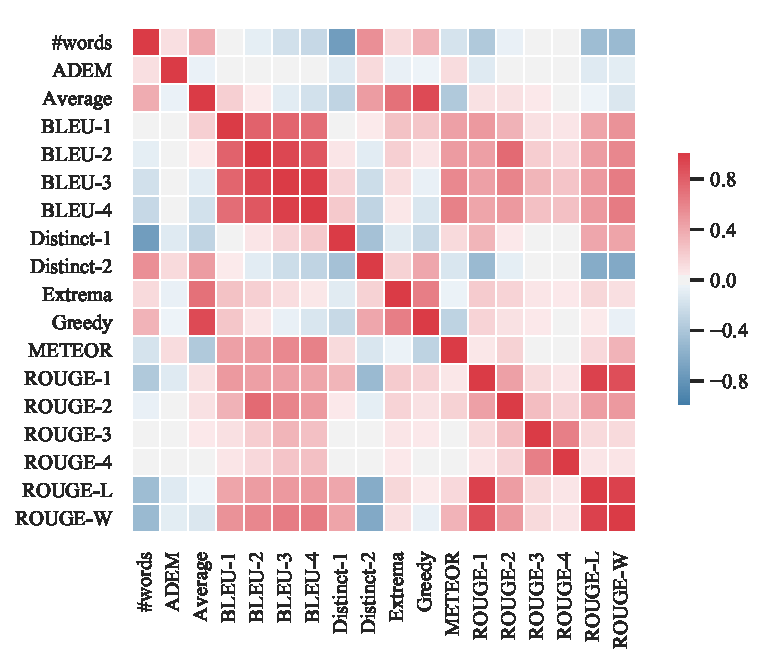
\includegraphics[width=\linewidth]{figure/plot/heatmap/v4/pearson/vhred/ubuntu/plot.pdf}
        \caption{(VHRED, Ubuntu)}
    \end{subfigure}
    \begin{subfigure}{0.35\linewidth}
        \centering
        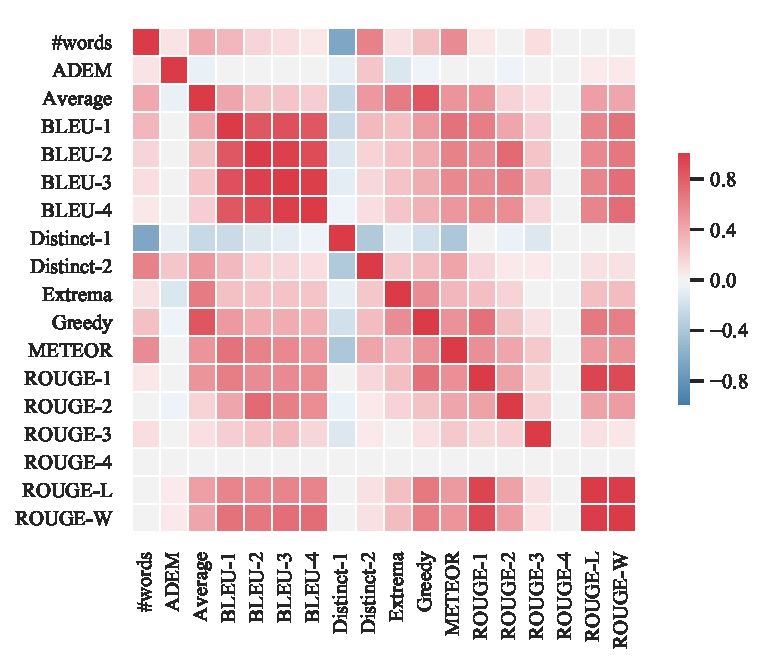
\includegraphics[width=\linewidth]{figure/plot/heatmap/v4/pearson/lstm/lsdscc/plot.pdf}
        \caption{(LSTM, LSDSCC)}
    \end{subfigure}%
    \begin{subfigure}{0.35\linewidth}
        \centering
        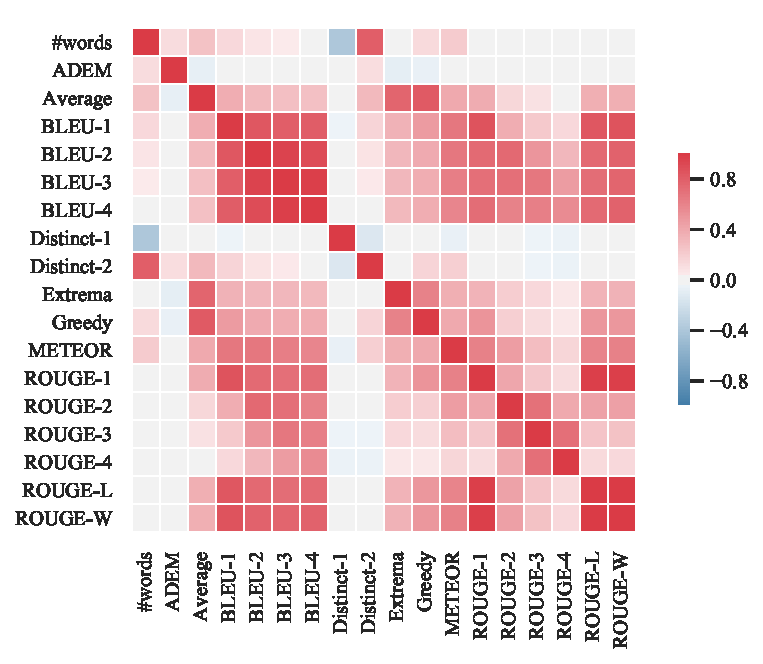
\includegraphics[width=\linewidth]{figure/plot/heatmap/v4/pearson/lstm/opensub/plot.pdf}
        \caption{(LSTM, OpenSubtitles)}
    \end{subfigure}%
    \begin{subfigure}{0.35\linewidth}
        \centering
        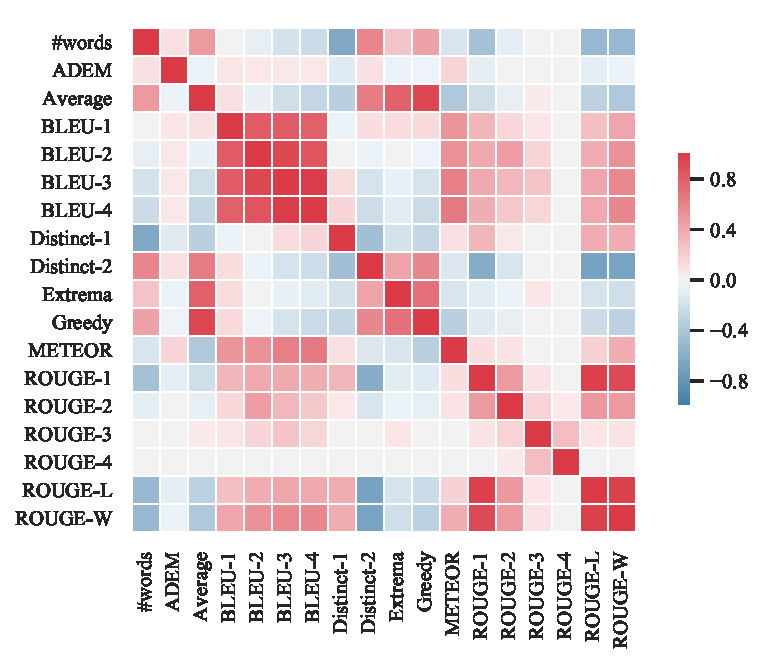
\includegraphics[width=\linewidth]{figure/plot/heatmap/v4/pearson/lstm/ubuntu/plot.pdf}
        \caption{(LSTM, Ubuntu)}
    \end{subfigure}
    \caption{Heatmaps of Pearson's r}
    \label{fig:corr_heatmap}
\end{figure}


    Each subfigure in Fi.g \ref{fig:corr_heatmap} is plotted from the correlation matrix for a model instance. The color of the cells represents the degree of correlation between the row and column labels, with red, blue, and white stand for positive, negative and zero correlation, respectively. One can spot red regions divided by white or blue lines from these plots, showing the signs of high local correlations.

    To better observe the agreement and disagreement among the metrics, we applied hierarchical clustering to the metrics based on their correlations and the results are shown in Fig. \ref{fig:hierarchy}. A hierarchical clustering algorithm starts with a forest of nodes and iteratively merges them into larger clusters until the root cluster is created. We used the following node-level distance $\textit{dist}(\cdot, \cdot)$ and cluster-level distance $d(\cdot, \cdot)$:
    \begin{align}
        \textit{dist}(i, j) &= 1 - \textit{corr}(i, j) \\
        d(u, v) &= \frac{\sum_{i,j}\textit{dist}(i, j)}{|u| \cdot |v|}
    \end{align}
    where $i$ and $j$ are points in cluster $u$ and $v$, respectively. $|u|$ and $|v|$ are the cardinalities of cluster $u$ and $v$, respectively\footnote{This is also known as the average method.}. Again the correlation is based on Pearson's r.
    \begin{figure}[htb]
    \begin{subfigure}{0.35\linewidth}
        \centering
        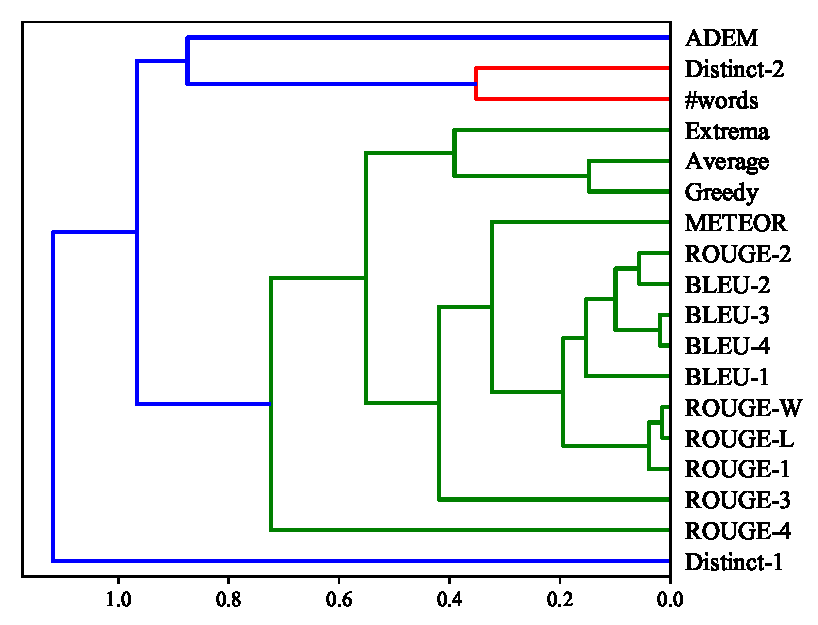
\includegraphics[width=\linewidth]{figure/plot/hierarchy/v3/pearson/hred/lsdscc/plot.pdf}
        \caption{(HRED, LSDSCC)}
    \end{subfigure}%
    \begin{subfigure}{0.35\linewidth}
        \centering
        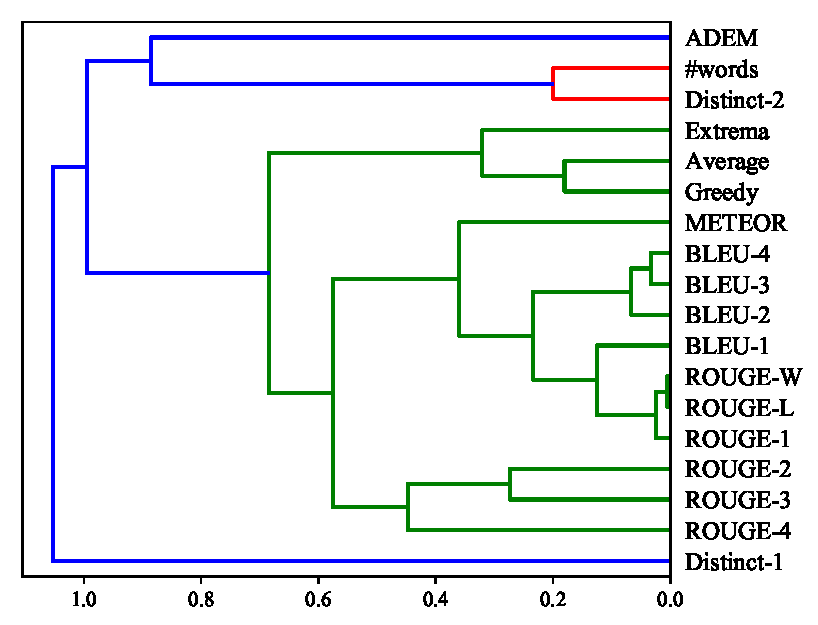
\includegraphics[width=\linewidth]{figure/plot/hierarchy/v3/pearson/hred/opensub/plot.pdf}
        \caption{(HRED, OpenSubtitles)}
    \end{subfigure}%
    \begin{subfigure}{0.35\linewidth}
        \centering
        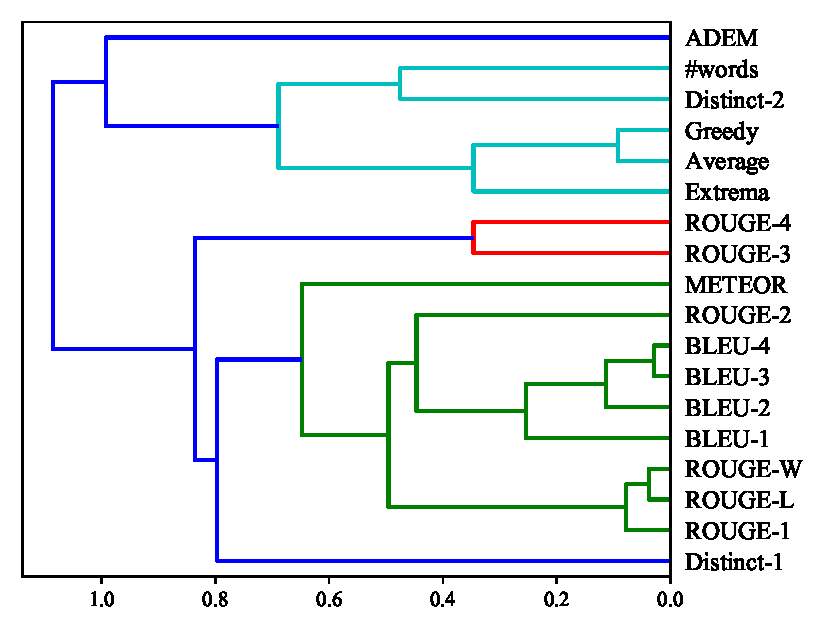
\includegraphics[width=\linewidth]{figure/plot/hierarchy/v3/pearson/hred/ubuntu/plot.pdf}
        \caption{(HRED, Ubuntu)}
    \end{subfigure}
    \begin{subfigure}{0.35\linewidth}
        \centering
        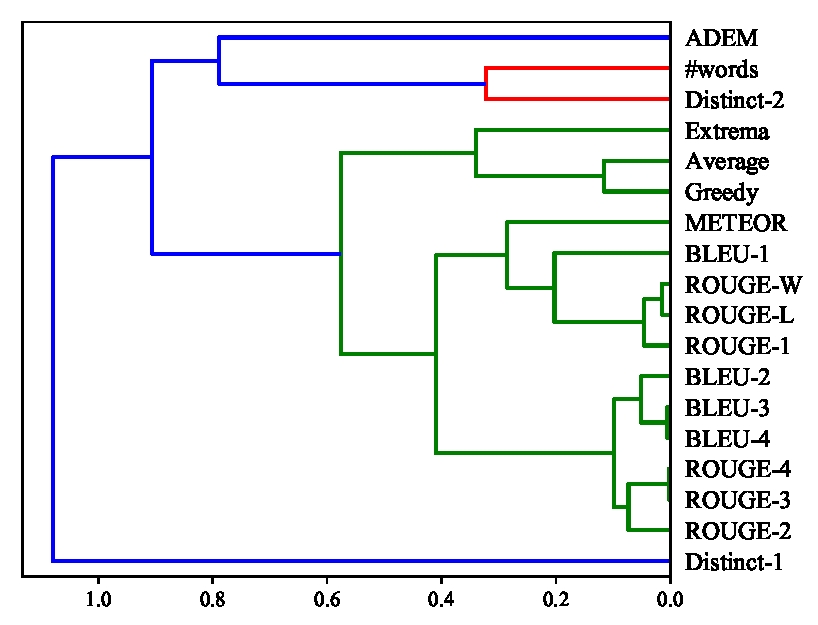
\includegraphics[width=\linewidth]{figure/plot/hierarchy/v3/pearson/vhred/lsdscc/plot.pdf}
        \caption{(VHRED, LSDSCC)}
    \end{subfigure}%
    \begin{subfigure}{0.35\linewidth}
        \centering
        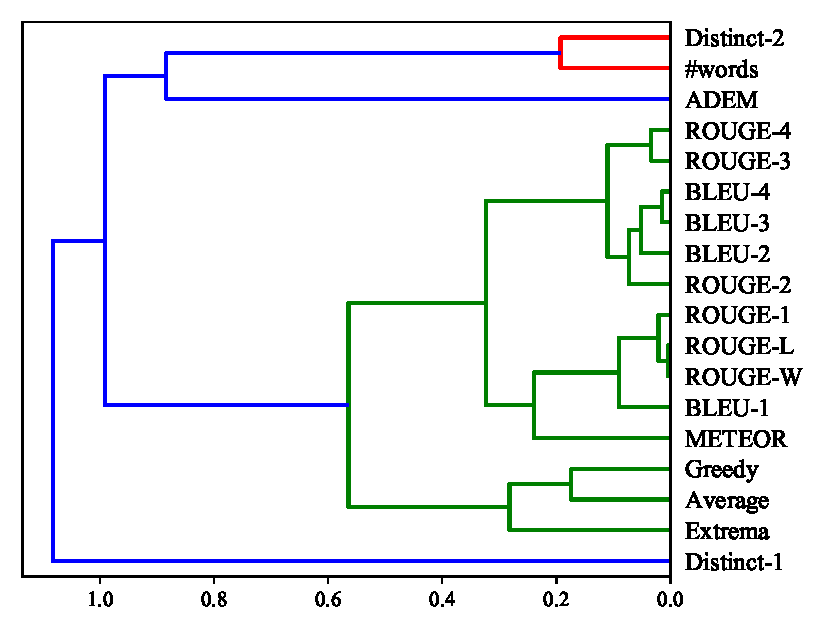
\includegraphics[width=\linewidth]{figure/plot/hierarchy/v3/pearson/vhred/opensub/plot.pdf}
        \caption{(VHRED, OpenSubtitles)}
    \end{subfigure}%
    \begin{subfigure}{0.35\linewidth}
        \centering
        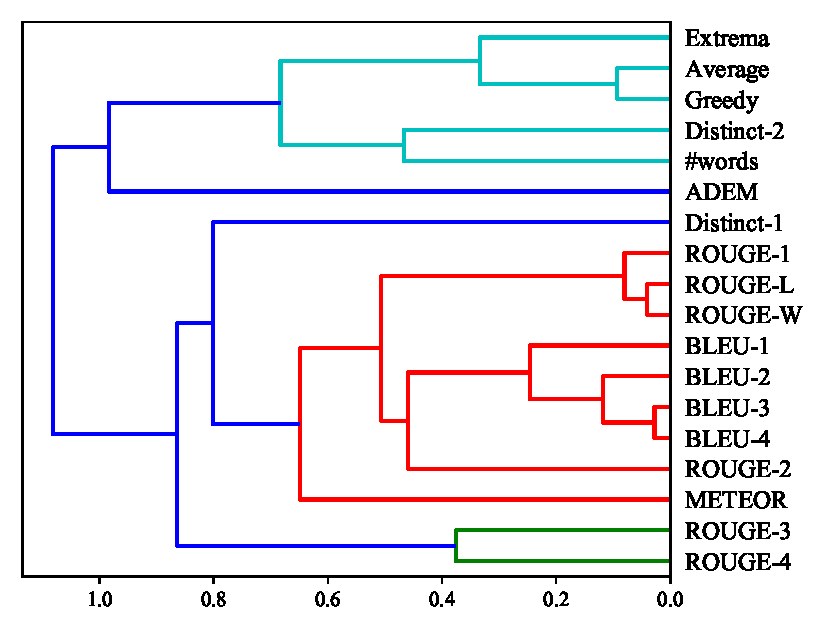
\includegraphics[width=\linewidth]{figure/plot/hierarchy/v3/pearson/vhred/ubuntu/plot.pdf}
        \caption{(VHRED, Ubuntu)}
    \end{subfigure}
    \begin{subfigure}{0.35\linewidth}
        \centering
        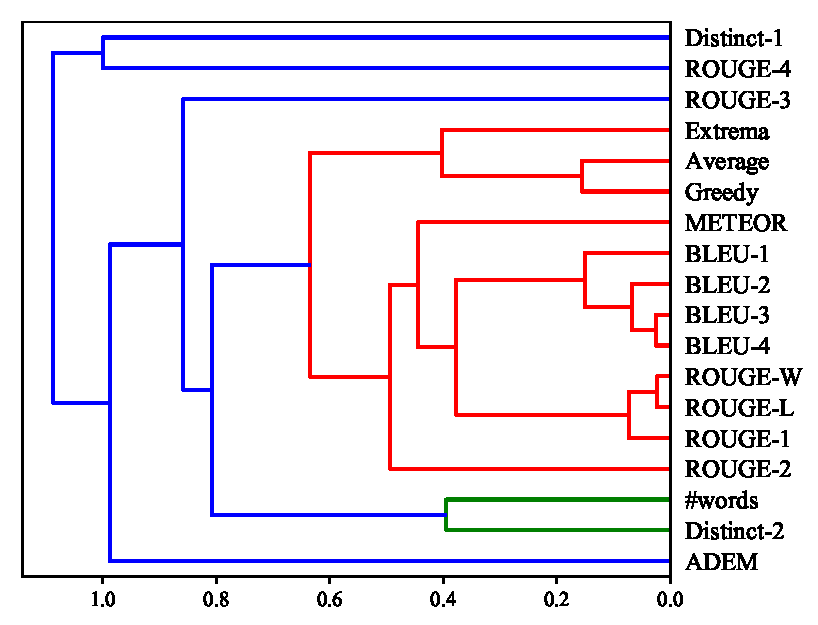
\includegraphics[width=\linewidth]{figure/plot/hierarchy/v3/pearson/lstm/lsdscc/plot.pdf}
        \caption{(LSTM, LSDSCC)}
    \end{subfigure}%
    \begin{subfigure}{0.35\linewidth}
        \centering
        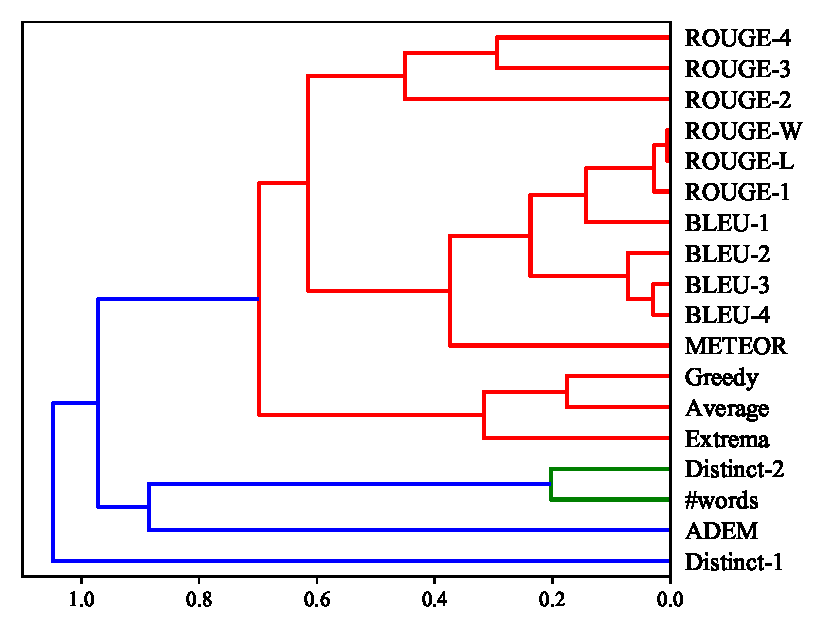
\includegraphics[width=\linewidth]{figure/plot/hierarchy/v3/pearson/lstm/opensub/plot.pdf}
        \caption{(LSTM, OpenSubtitles)}
    \end{subfigure}%
    \begin{subfigure}{0.35\linewidth}
        \centering
        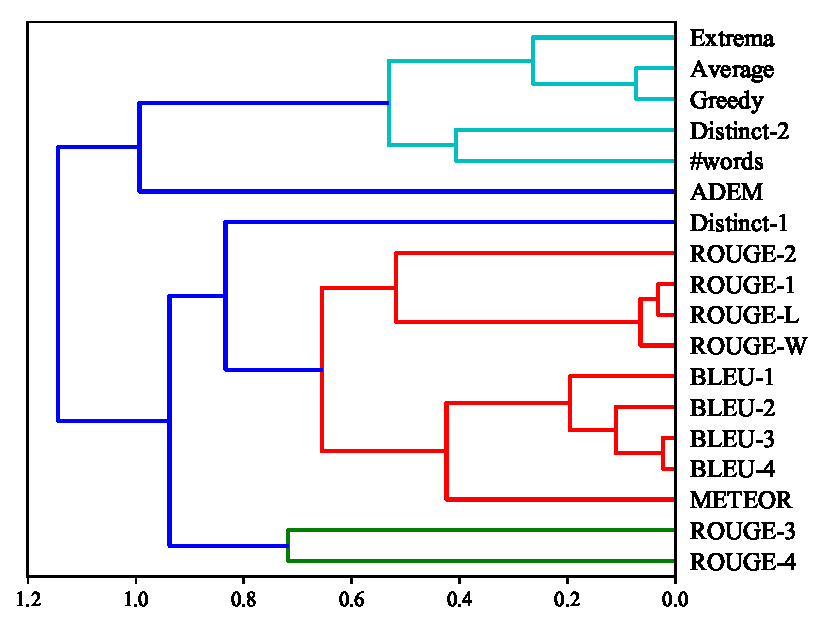
\includegraphics[width=\linewidth]{figure/plot/hierarchy/v3/pearson/lstm/ubuntu/plot.pdf}
        \caption{(LSTM, Ubuntu)}
    \end{subfigure}
    \centering
    \caption{Hierarchical Clustering with Pearson's r}
    \label{fig:hierarchy}
\end{figure}


    From Fig. \ref{fig:hierarchy}, we observe a hierarchy of agreement among different metrics. The clusters that were created in the earlier iterations appear closer to the leaves of the tree, which indicates higher pairwise correlations or stronger inter-metric agreement. As a cluster grows larger, its children become loosely connected with greater distances. It is interesting to find that the dendrograms in Fig. \ref{fig:hierarchy} share some regular structure, which has an observable correspondence to the category of the metrics. Across all the settings, we generally observe these independent clusters, named after their shared category or a representative element:
    
    1) Word-Overlap: a large cluster that contains many subclusters formed by different word-overlap metrics, such as BLEU, ROUGE, and METEOR.
       
    2) Word-Embedding: a small cluster that contains Vector-Average, Vector-Extrema, and Greedy-Matching.
      
    3) ADEM: a standalone cluster formed by ADEM.
    
    4) Distinct-1: a metric that might belong to some cluster or become a standalone cluster depending on the dataset involved.
       
    5) Distinct-2 and \#words: a generally observable cluster.

    Those clusters confirm our hypothesis on the inconsistency among different metrics. Luckily, there are still some forms of agreement that the same cluster of metrics can reach. Unfortunately, the exact reasons why the clusters are formed this way are unclear to us. Although our experiments have a simple procedure, it should be noted that the mechanism behind each step has a complex nature. For example, the dialogue datasets are intrinsically very diverse and the way the generative models work is not well-understood. Besides, it is also unclear how these metrics reflect the desirable properties of a response. Hence we can only conclude that similar metrics tend to have consistent results on the example-level. The similarity of metrics generally refers to their mechanisms, such as the way to extract overlap units or derive semantics from an utterance, or the way to combine different components.

    Specifically, on the one hand, we find that metrics based on word overlap tend to have high pairwise correlations since they all make use of the n-gram statistics somehow. On the other hand, it is confirming to observe that ADEM does not correlate with all the other metrics since it has a much higher correlation with human judgment while other metrics do not.

    \subsection{Qualitative Analysis}
    \begin{table}[h]
    \caption{An Example from OpenSubtitles}
    \label{tab:Example_OpenSubtitles}
    \centering
    \begin{tabular}{|l|*{3}{p{0.2\textwidth}|}}
        \hline
        Context & \multicolumn{3}{p{0.64\textwidth}|}{You will be in classes does she know that? As if you' re gonna have all this free time to pal around with her.} \\
        \hline
        Reference & \multicolumn{3}{p{0.64\textwidth}|}{okay sure we il start there. \\
        \hline
        Model & LSTM & HRED & VHRED \\
        \hline
        Response & C all this time. & Her room starts in half 50 percent. & I figured this was gonna be a fun stretch. \\
        \hline
        ADEM & 2.5987 & \textbf{2.6411} & 2.6276 \\
        \hline
        BLEU-1 & 0 & 0 & 0 \\
        \hline
        Distinct-1 & 1.0 & 1.0 & 1.0 \\
        \hline
        Distinct-2 & 0.75 & 0.8571 & \textbf{0.8889} \\
        \hline
        Greedy & \textbf{0.3520} & 0.2336 & 0.3412 \\
        \hline
        Average & 0.4979 & 0.3468 & \textbf{0.6607} \\
        \hline
        Extrema & 0.2791 & 0.1341 & \textbf{0.3995} \\
        \hline
        METEOR & 0 & \textbf{0.0105} & 0 \\
        \hline
        ROUGE-L & 0 & 0 & 0 \\
        \hline
        ROUGE-W & 0 & 0 & 0 \\
        \hline
        \#words & 4 & 7 & \textbf{9} \\
        \hline
    \end{tabular}
\end{table}

    Table \ref{tab:Example_OpenSubtitles} serves as an example of the inter-metrics inconsistency. The response from HRED mentions ``her room'', which is relevant to the subject ``she'' in the context and the verb ``starts'' matches the ``start'' in the reference. The response from VHRED does not share any token with the context or reference, but it remarks the event mentioned by the context so it is quite a reasonable one.

    All three responses share no n-grams with either the context or the reference in terms of exact matching. Thus, all the word-overlap metrics yield a zero value. However, all the word-embedding metrics give non-zero value, making them incompatible with the word-overlap metrics.

    In terms of semantic relevance, the responses from both HRED and VHRED are somehow related to the topic of the dialogue, while the response from LSTM looks grammatically incomplete. One will mostly agree that the responses from HRED and VHRED are equally better than that from LSTM. However, the ranks given by the word-embedding metrics do not agree with the manual inspection. For example, they all give higher scores to LSTM than HRED.

    \section{Conclusion and Future Work}
    In this paper, we followed the work of \cite{HowNot} and try to understand the reasons behind low metric-human correlations. We investigated the system-level scores and leveraged statistical analyses to reveal the inter-metrics correlation on the example level. Our study shows a high consistency of metrics on the system level, as shown by others \cite{HowNot,VHRED,GoogleChatbot}. We further show that on the example level, similar metrics tend to score the examples more consistently and the degree of correlations forms a hierarchical cluster.

    Intuitively, different metrics judge a dialogue from different angles, while human beings judge it from a quite comprehensive perspective. This might explain why the metrics do not correlate well with human judgments. Our discovery of the example-level correlation-based hierarchical clusterings of metrics is a novel contribution.

    Based on the observations, it is recommended to avoid using a set of metrics that have low pairwise correlations since that will make the example-level scores divergent and hard to explain. We also urge against the use of metrics that are known to have poor correlations with human judgments. In the future, we would like to look deeper into the mechanisms behind the metric-human correlations.


 %   \subsection*{Acknowledgements.}
 %   This work was supported by the Engineering Research Center of Ministry of Education for Advanced Computer Application Technology (ACAREC) of Beihang University. We also appreciate the advice from anonymous reviewers.

    \bibliographystyle{splncs04}
    \bibliography{reference}
\end{document}
